%!TEX root=../main.tex
\section{On the geometry of multivariate functional data} % (fold)
\label{sec:geometric_point_of_view_mfpca}

\subsection{Duality diagram} % (fold)
\label{sub:duality_diagram}

\begin{figure}
    \centering
    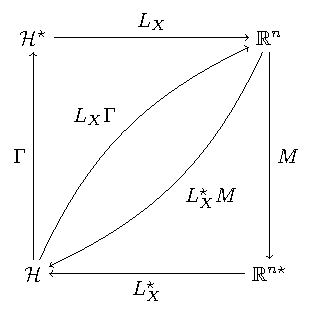
\includegraphics[scale=1.2]{figures/duality_diagram.pdf}
    \caption{Duality diagram}
    \label{fig:duality_diagram}
\end{figure}


% subsection duality_diagram (end)

\subsection{Cloud of individuals} % (fold)
\label{sub:cloud_of_individuals}

Given $n \in \{1, \dots, N\}$, let $\{\Xnp(t_p),\,t_p \in \TT{p},\,p = 1, \dots, P\}$ be the features set for a particular observation $n$. We identify this set as the point $\pobs{M}_n$ in the space $\HH$. The space $\HH$ is referred to as the observations' space. The cloud of points that represents the set of observations in $\HH$ is denoted by $\CN$. Let $\GN$ be the centre of gravity of the cloud $\CN$. In the space $\HH$, its coordinates are given by $\{\mup{p}(t_p),\,t_p \in \TT{p},\,p = 1, \dots, P\}$. If the features are centered, the origin $\OH$ of the axes in $\HH$ coincides with $\GN$.

\begin{figure}
    \centering
    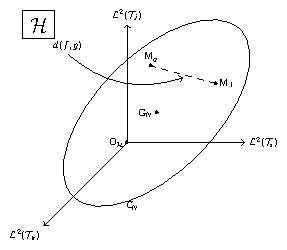
\includegraphics[scale=1.2]{figures/cloud_obs.pdf}
    \caption{Cloud of observations. The observation $f$ (resp. $g$) is identified by the point $\pobs{M}_f$ (resp. $\pobs{M}_g$) in the cloud $\CN$. The point $\GN$ is the center of gravity of $\CN$ and the point $\OH$ is the origin of the space $\HH$.}
    \label{fig:cloud_obs}
\end{figure}

Let $f$ and $g$ be two elements in $\HH$ and denote by $\pobs{M}_f$ and $\pobs{M}_g$ their associated points in $\CN$ (see Figure~\ref{fig:cloud_obs}). The distance between these observations is defined as
\begin{equation}\label{eq:distance_obs}
    d^2(f, g) = \normH{f - g}^2 = \sum_{p = 1}^P \int_{\TT{p}}\left\{\fp(t_p) - \gp(t_p)\right\}^2 \dd t_p.
\end{equation}
This distance measures how different the observations are, and thus characterizes the shape of the cloud $\CN$. Another description of this shape is to consider the distance between each observation and $\GN$, the center of the cloud. Let $f$ be an element of $\HH$, associated to the point $\pobs{M}_f$, and $\mu$ the element of $\HH$ related to $\GN$, the distance between $f$ and $\mu$ is given by
\begin{equation}\label{eq:distance_center}
    d^2(f, \mu) = \normH{f - \mu}^2 = \sum_{p = 1}^P \int_{\TT{p}}\left\{\fp(t_p) - \mup{p}(t_p)\right\}^2 \dd t_p.
\end{equation}
Given the set $\XX$, the total inertia of $\CN$, with respect to $\GN$, is given by
\begin{equation}\label{eq:inertia}
    \sum_{n = 1}^N \pi_n d^2(X_n, \mu) = \frac{1}{2}\sum_{i = 1}^N \sum_{j = 1}^N \pi_i \pi_j d^2(X_i, X_j) = \sum_{p = 1}^P \int_{\TT{p}}\Var{\Xp{p}(t_p)} \dd t_p.
\end{equation}
The derivation of these equalities are given in Appendix \ref{sec:derivation_of_the_inertia_of_the_clouds}.

\begin{remark}
    These results have the same interpretation as for multivariate scalar data. This is also the multivariate analogue of the relation between variance and sum of squared differences known for univariate functional data. If the features are reduced beforehand, the total inertia of the cloud $\CN$ is equal to the number of components $P$. We are, in general, not interested by the total inertia but mostly how this variance is spread among the features.
\end{remark}

% subsection cloud_of_individuals (end)

\subsection{Cloud of features} % (fold)
\label{sub:cloud_of_features}

\textcolor{red}{For now, we need that all the features are defined on the same space $\TT{0}$.
Let $\{\Xnp(t), n = 1, \dots, N\}$ be the observations set for a particular feature $p$. We identify this set as the point $\mathsf{M}_p$ in the space $\GG \coloneqq \sLp{\TT{0}}^N$. The set $\GG$ is refered as the features' space, or variables' space. The cloud of points that represents the set of features is denoted by $\CP$. Let $\OG$ be the centre of this space. Its coordinates are given by a vector of functions of length $N$ where each entry is $f(t) = 0$ for all $t \in \TT{0}$.
We assume that the observations are centered. Consider $\mathsf{M}_h$ a point in $\CP$ and $h$ the element of $\GG$ representing by $\mathsf{M}_h$. Let $o$ be the element of $\OG$ representing by $\OG$. The distance between $\mathsf{M}_h$ and $\OG$ is defined as
\begin{equation*}
d^2(h, o) = \sum_{n = 1}^N p_n \normLp{h_n - \mu_h}^2 = \int_{\TT{0}} \Var h^{(p)}(t)dt.
\end{equation*}
}

\begin{figure}
    \centering
    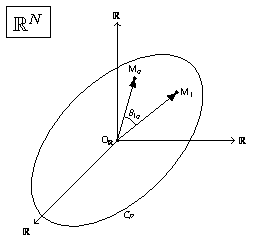
\includegraphics[scale=1.2]{figures/cloud_features.pdf}
    \caption{Cloud of features.}
    \label{fig:cloud_features}
\end{figure}
% subsection cloud_of_features (end)

\subsection{On centering and reducing} % (fold)
\label{sub:on_centering_and_reducing}

For conducting an MFPCA, the features are usually assumed centred \citep{happMultivariateFunctionalPrincipal2018a}. \cite{protheroNewPerspectivesCentering2021} give a complete overview of centering in the context of FDA. Here, we comment on the geometric interpretation of centering in this context and compare with the multivariate scalar case. We focus on the usual centering in FDA, namely $\Xnp(t_p) - \mu^{(p)}(t_p),~t_p \in \TT{p}$ (refered as \emph{object centering} in \cite{protheroNewPerspectivesCentering2021}).
The geometric interpretation of the centering differs if we refer to the observations' space $\HH$ or the features' space $\GG$. Within the space $\HH$, centering is interpreted as translating the centre of gravity of the curves $\GN$ to the origin point $\OH$ of $\HH$. This transformation, being a translation, does not change the shape of the cloud $\CN$. The interpretation is the same as for the multivariate scalar data. Within the space $\GG$, the centering is harder to interpret and does not have the same meaning as in the multivariate case. Actually, in the multivariate scalar case, the centering of the data can be geometrically interpreted as the projection of the data on the subspace orthogonal to the constant vector. However, what happens if we project the multivariate curves onto the vector (of length $P$) of constant functions?


\textcolor{red}{In the space $\GG$, the inner product is given by
\begin{equation}
\inH{f}{g} = \sum_{i = 1}^N \int_{\TT{k}} f^{(k)}_i(t)g^{(k)}_i(t)dt, \quad f, g \in \GG.
\end{equation}
Let $\mathbf{1}$ be the vector of constant function in $\GG$ and $f$ an element of $\GG$. The projection of $f$ onto $\mathbf{1}$ is then given by
\begin{equation}
P_{\mathbf{1}}f = \frac{\inH{f}{\mathbf{1}}}{\normH{\mathbf{1}}}\mathbf{1} = \frac{1}{N\lvert \TT{k} \rvert}\sum_{n = 1}^N \int_{\TT{k}} f^{(k)}_n(t)dt\mathbf{1}
\end{equation}
In practice, this is equivalent to computing the mean value of the mean curve for each component, referred as \emph{grand mean centering} in \cite{protheroNewPerspectivesCentering2021}.}

Concerning the standardization of the data, there are mainly two proposal in the literature. \cite{happMultivariateFunctionalPrincipal2018a} propose to weight each component $p$ by
\begin{equation}
w_p = \left(\int_{\TT{p}} \Var X^{(p)}(t_p) \dd t_p\right)^{-1}.
\end{equation}
This standardization is coherent with the derivation of the total inertia of the observations' space. Using these weights, the total inertia of $\CN$ is equal to the number of components $P$. \cite{chiouMultivariateFunctionalPrincipal2014} propose to standardize each component $p$ of the data using the function
\begin{equation}
w_p(t_p) = \left(\Var X^{(p)}(t_p)\right)^{-1/2}, \quad t_p \in \TT{p}.
\end{equation}
This corresponds to a standardization of the curves by the standard deviation of the component at each sampling point. The standard deviation curve is estimated as the square root of the diagonal of the covariance function estimates, obtained using a local linear smoother of the pooled data. 

% subsection on_centering_and_reducing (end)

% section sec:geometric_point_of_view_mfpca (end)